\section {Caractéristique de l'acide benzoïque}
\textbf{Source du sujet :} Baccalauréat de mars 2023 – exercice 4 du sujet de Métropole.

\subsection{Introduction}
L'acide benzoïque, de formule \ce{C6H5COOH}, et le benzoate de sodium sont des conservateurs antimicrobiens
respectivement identifiés par les codes E210 et E211. Ils sont présents dans de nombreux produits alimentaires
et notamment dans certaines boissons gazeuses sucrées. À température ambiante, l’acide benzoïque est un solide blanc.

\begin{figure}[h]
    \centering
    \chemfig{OH-[:120,,1](=[:60]O)-[:180]=_[:240]-[:180]=_[:120]-[:60]=_(-[:300])}
    \caption{Formule topologique de l’acide benzoïque}
\end{figure}

\textbf{Données :}
\begin{itemize}
    \item Masse molaire de l'acide benzoïque : $M = \SI{122}{\gram\per\mole}$.
    \item Température de fusion de l'acide benzoïque : $\theta_f = \SI{122,4}{\degreeCelsius}$.
    \item pKa du couple acide benzoïque/ion benzoate : $pKa = 4,2$.
    \item Le benzoate de sodium est soluble dans l’eau.
\end{itemize}

\begin{table}[h]
\centering
\begin{tabular}{|c|c|c|c|c|}
\hline
 & Densité & Eau & Éthanol & Éther éthylique \\
\hline
Acide benzoïque & - & Peu soluble & Très soluble & Très soluble \\
\hline
Eau & 1,0 & - & Miscible & Non miscible \\
\hline
Éthanol & 0,76 & Miscible & - & - \\
\hline
Éther éthylique & 0,71 & Non miscible & - & - \\
\hline
\end{tabular}
\caption{Tableau de solubilité des substances}
\end{table}

L’objectif de cet exercice est de vérifier l’indication d’une étiquette de boisson gazeuse concernant la
présence d’un conservateur.

\subsection{Questions}

\begin{questionmult}{acidbenzo1}
    Entourer et nommer le groupe caractéristique présents dans la formule topologique de l'acide benzoïque ci-dessous.\\
        \centering\chemfig{OH-[:120,,1](=[:60]O)-[:180]=_[:240]-[:180]=_[:120]-[:60]=_(-[:300])}\\
    \AMCOpen{}{
        \mauvaise{NA}\scoring{b=0}
        \bonne{Groupe identifié}\scoring{b=.5}
        \bonne{Groupe nommé}\scoring{b=.5}
    }
    \explain{Le groupe caractéristique est le groupe carboxyle (--COOH). Dans la formule topologique, il est
    identifiable par le carbone lié à un oxygène par une double liaison et à un groupe hydroxyle (--OH).}
\end{questionmult}

\begin{question}{acidbenzo2}
    Écrire la formule topologique de l’ion benzoate, base conjuguée de l’acide benzoïque.\\
    \begin{EnvQuadrillage}[NbCarreaux=20x4,Grille=Seyes,Marge=1]
    \end{EnvQuadrillage}
    \AMCOpen{}{
        \mauvaise{NA}\scoring{b=0}
        \mauvaise{$\approx$}\scoring{b=.5}
        \bonne{OK}\scoring{b=1}
    }
    \explain{La formule topologique de l’ion benzoate est :
    \chemfig{\mcfright{O}{^{\mcfminus}}-[:120](=[:60]O)-[:180]=^[:120]-[:180]=^[:240]%
-[:300]=^(-[:60])}. La charge négative est portée par l’oxygène du groupe carboxylate.}
\end{question}

\begin{question}{acidbenzo3}
    Représenter le diagramme de prédominance du couple acide benzoïque/ion benzoate.\\
    \begin{EnvQuadrillage}[NbCarreaux=20x3,Grille=Seyes,Marge=1]
    \end{EnvQuadrillage}
    \AMCOpen{}{
        \mauvaise{NA}\scoring{b=0}
        \mauvaise{$\approx$}\scoring{b=.5}
        \bonne{OK}\scoring{b=1}
    }
    \explain{Le diagramme de prédominance doit montrer :
    - À un pH inférieur à 4,2, l’acide benzoïque (\ce{C6H5COOH}) est prédominant.
    - À un pH supérieur à 4,2, l’ion benzoate (\ce{C6H5COO-}) est prédominant.
    \begin{center}
        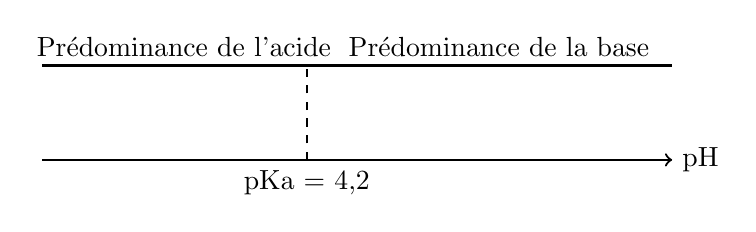
\begin{tikzpicture}[scale=0.8]
            \draw[->, thick] (0,0) -- (10,0) node[right] {pH};
            \draw[thick] (0,1.5) -- (10,1.5);
            \draw[thick, dashed] (4.2,0) node[below] {pKa = 4,2} -- (4.2,1.5);
            \node at (2.25,1.8) {Prédominance de l’acide};
            \node at (7.25,1.8) {Prédominance de la base};
        \end{tikzpicture}
    \end{center}}
\end{question}

\subsection{Expériences}

Dans un premier temps, on réalise deux expériences permettant de mettre en évidence les propriétés de l’acide
benzoïque et de l’ion benzoate :
\begin{itemize}
\item Expérience (1) : Dans un tube à essais contenant une solution de benzoate de sodium, on ajoute quelques
gouttes d’acide chlorhydrique concentré. On observe qu’un solide blanc apparaît.
\item Expérience (2) : Dans un tube à essais contenant une solution de soude concentrée, on ajoute de l’acide
benzoïque solide. On observe que le solide introduit disparaît.
\end{itemize}

\begin{questionmult}{acidbenzo4}
    On donne l'équation chimique suivante :\\
    \ce{C6H5COO^-_{(aq)} + H3O^+_{(aq)} -> C6H5COOH_{(aq)} + H2O_{(l)}}\\
    La réaction qui correspond à l'équation ci-dessus modélise une transformation chimique ayant lieu lors de l’une
    des expériences précédentes. Indiquer, en justifiant la réponse, s'il s'agit de l'expérience (1) ou de l'expérience (2).
    \begin{EnvQuadrillage}[NbCarreaux=20x6,Grille=Seyes,Marge=1]
    \end{EnvQuadrillage}
    \AMCOpen{}{
        \mauvaise{NA}\scoring{b=0}
        \bonne{Expérience identifiée}\scoring{b=0.5}
        \bonne{Justification correcte}\scoring{b=0.5}
    }
    \explain{Il s’agit de l’expérience (1). Les réactifs sont l’ion benzoate (\ce{C6H5COO-}) et l’ion oxonium (\ce{H3O+}).
    Ces ions sont présents dans l’expérience 1, où l’acide chlorhydrique apporte les ions \ce{H3O+}.}
\end{questionmult}

L’étiquette d’une boisson gazeuse indique qu’elle contient du benzoate de sodium comme conservateur alimentaire,
entre autres, et on souhaite vérifier cette indication. On réalise pour cela une extraction liquide-liquide.
On suit le protocole expérimental suivant :

\begin{enumerate}
    \item Verser 500 mL de boisson dans un grand bécher.
    \item Ajouter de l’acide chlorhydrique jusqu’à amener le pH à environ 2.
    \item Ajouter alors 40 mL d’éther éthylique, agiter et laisser reposer.
    \item Transvaser l’ensemble dans une ampoule à décanter.
    \item Agiter vigoureusement pendant deux minutes en prenant soin de dégazer régulièrement pour éviter toute surpression.
    \item Laisser décanter.
    \item Récupérer la phase aqueuse S dans un bécher et la phase organique dans un erlenmeyer.
\end{enumerate}

\begin{question}{acidbenzo5}
    Préciser ce qu'il se passe lors de l'étape 2 du protocole.
    \begin{EnvQuadrillage}[NbCarreaux=20x5,Grille=Seyes,Marge=1]
    \end{EnvQuadrillage}
    \AMCOpen{}{
        \mauvaise{NA}\scoring{b=0}
        \mauvaise{$\approx$}\scoring{b=.5}
        \bonne{OK}\scoring{b=1}
    }
    \explain{Lors de l’étape 2, l’ion benzoate (\ce{C6H5COO-}) se transforme en acide benzoïque (\ce{C6H5COOH})
    sous l’effet de l’ajout d’acide chlorhydrique. Le pH est abaissé à 2, ce qui est inférieur au pKa du couple
    (4,2), favorisant la forme acide.}
\end{question}

\begin{question}{acidbenzo6}
    À l'aide des données, expliquer pourquoi l'éther éthylique constitue un solvant extracteur plus adapté que
    l'éthanol lors de la réalisation de l'étape 3 du protocole.
    \begin{EnvQuadrillage}[NbCarreaux=20x6,Grille=Seyes,Marge=1]
    \end{EnvQuadrillage}
    \AMCOpen{}{
        \mauvaise[F]{NA}\scoring{b=0}
        \mauvaise[C]{$\approx$}\scoring{b=.5}
        \bonne[C]{OK}\scoring{b=1}
    }
    \explain{L’éther éthylique est non miscible à l’eau et l’acide benzoïque y est très soluble. À l’inverse, l’éthanol
    est miscible à l’eau, ce qui rendrait l’extraction inefficace. L’éther éthylique permet donc une séparation
    nette des phases organique et aqueuse.}
\end{question}

\begin{questionmult}{acidbenzo7}
    Compléter le schéma ci-dessous, en justifiant, à l'aide des données, la nature
    et la position des différentes phases dans l'ampoule à décanter à l'issue de l'étape 6 du protocole.

    \begin{center}
        \begin{minipage}[t]{0.3\textwidth}
            \centering
            \includegraphics[height=5cm, keepaspectratio]{images/ste5_ampoule.png}
        \end{minipage}%
        \begin{minipage}[t]{0.7\textwidth}
            \begin{EnvQuadrillage}[NbCarreaux=14x6, Grille=Seyes,Marge=1]
            \end{EnvQuadrillage}
        \end{minipage}
    \end{center}

    \AMCOpen{}{
        \mauvaise[F]{NA}\scoring{b=0}
        \bonne[C]{ScBuoy}\scoring{b=.5}
        \bonne[C]{ScAcd}\scoring{b=.5}
        \bonne[C]{XpBuoy}\scoring{b=.5}
        \bonne[C]{Ovl}\scoring{b=.5}
   }
    \explain{L’éther éthylique (densité = 0,71) est moins dense que l’eau (densité = 1,0). La phase organique (éther)
    constitue donc la phase supérieure, tandis que la phase aqueuse, plus dense, est la phase inférieure.
    \centering
    \includegraphics[height=5cm, keepaspectratio]{images/ste5_ampoule_corr.png}}
\end{questionmult}

\begin{question}{acidbenzo8}
    Après évaporation du solvant extracteur, il reste une masse \qty{10.0}{\milli\gram} de solide blanc. Proposer
    une méthode expérimentale permettant de vérifier que ce solide blanc est bien de l'acide benzoïque.
    \begin{EnvQuadrillage}[NbCarreaux=20x4,Grille=Seyes,Marge=1]
    \end{EnvQuadrillage}
    \AMCOpen{}{
        \mauvaise[F]{NA}\scoring{b=0}
        \mauvaise[B]{$\approx$}\scoring{b=.5}
        \bonne[A]{OK}\scoring{b=1}
   }
    \explain{On peut mesurer son point de fusion au banc Kofler. La température de fusion de l’acide benzoïque
    est donnée dans l’énoncé : \qty{122.4}{\degreeCelsius}. Si le solide fond à cette température, il s’agit bien
    d’acide benzoïque.}
\end{question}

\begin{questionmult}{acidbenzo9}
    Sachant que la concentration $C$ en quantité de matière totale théorique d'ions benzoate dans cette
    boisson est égale à \qty{4.0e-4}{\mol\per\litre}, montrer que la masse théorique d'acide
    benzoïque que l'on devrait obtenir à l'issue de l'extraction est égale à \qty{24}{\mg}.

    \begin{EnvQuadrillage}[NbCarreaux=20x8,Grille=Seyes,Marge=1]
    \end{EnvQuadrillage}

    \AMCOpen{}{
        \mauvaise{NA}\scoring{b=0}
        \bonne{Idée}\scoring{b=.5}
        \bonne{Forml}\scoring{b=.5}
        \bonne{Nb}\scoring{b=.5}
        \bonne{Ovl}\scoring{b=.5}
    }

    \explain{La masse théorique d’acide benzoïque est calculée comme suit :
    \[
    m = C \times V \times M = \SI{4.0e-4}{\mol\per\litre} \times \SI{0.5}{\litre} \times \SI{122}{\gram\per\mol} = \SI{24}{\mg}.
    \]
    La concentration $C$ est donnée, le volume $V$ est de 500 mL (0,5 L), et la masse molaire $M$ est de
    \SI{122}{\gram\per\mol}.}
\end{questionmult}

\begin{questionmult}{acidbenzo10}
    Le rendement d'une extraction étant défini comme le rapport de la masse de substance réellement extraite sur la
    masse théorique de substance que l'on aurait pu extraire, calculer le rendement de cette extraction et
    l'exprimer en pourcentage. Commenter ce résultat.
    \begin{EnvQuadrillage}[NbCarreaux=20x4,Grille=Seyes,Marge=1]
    \end{EnvQuadrillage}
    \AMCOpen{}{
        \mauvaise[F]{NA}\scoring{b=0}
        \bonne[C]{Idée}\scoring{b=.5}
        \bonne[B]{Forml}\scoring{b=.5}
        \bonne[A]{Nb}\scoring{b=.5}
        \bonne[A]{Ovl}\scoring{b=.5}
    }
    \explain{Le rendement est calculé comme suit :
    \[
    \eta = \frac{10,0}{24} \times 100 = 41,7\%.
    \]
    Ce rendement est relativement faible. Pour l’améliorer, il faudrait extraire une deuxième fois la phase
    aqueuse avec 40 mL d’éther éthylique, puis rassembler les phases organiques.}
\end{questionmult}
